\section{Разработка библиотеки для синтаксического анализа графов}
\subsection{Библиотека Meerkat}
Meerkat — это библиотека парсер-комбинаторов, разработанная на языке программирования Scala Али Афрузе и Анастасией Измайловой~\cite{IzmCombinator}. Библиотека предназначена для синтаксического анализа строк. Анализ, при использовании библиотеки, осуществляется за $O(n^3)$, где n – длина последовательности, а также осуществляет построение компактного представления леса разбора Binarized Shared Packed Parse Forest (BSPPF). В ней решены проблемы левой рекурсии, а также экспоненциальной сложности за счет использования техники мемоизации и Continuation-Passing Style, предложенной Марком Джонсоном~\cite{MemoizationInTopDown}.

\subsection{Распознаватель в стиле парсер-комбинаторов}
В терминах данной библиотеки базовый распознователь – это функция типа $Recognizer$, которая определяется как функция $Int => Result[Int]$ (принимает тип $Int$ и возвращает тип $Result[Int]$). Базовый распознаватель — это частичная функция, он принимает как аргумент позицию во входном потоке и возвращает значение $success$, соответствующее успешному разбору и содержащее следующую позицию, или значение $failure$, соответствующее ошибке при анализе.

Для составления любой КС-грамматики необходимо реализовать функциональность, который бы позволил реализовывать синтаксический анализатор терминала и пустой строки, а также функциональность, который бы позволил бы их объединять в последовательности и составлять правила. В библиотеке Meerkat для этих целей реализованы анализаторы $terminal$, и $epsilon$, а так же комбинаторы $seq$ и $rule$ (см. листининг~\ref{parserAll}).

\begin{listing}
\caption{Распознаватели в стиле парсер-комбинаторов}
\label{parserAll}
\centering
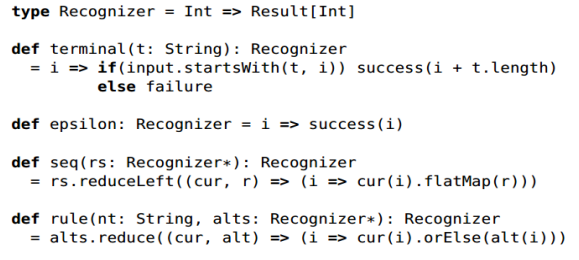
\includegraphics[width=0.9\textwidth]{Smolina/pics/combinators.png}
\end{listing}

Анализаторы представляют собой базовые распознаватели для терминала и пустой строки. Анализатор $terminal$ возвращает распознаватель, который принимает индекс текущей строки и возвращает $success$ в случае, когда суффикс строки с текущего символа равен значению терминала. Входной поток в данном случае предполагается глобальной переменной, но в реализации передаётся как параметр функции. 

Комбинатор $seq$ представляет собой последовательную композицию распознавателей. Он получает на вход текущую позицию и список распознавателей, затем применяет последовательно каждый из распознавателей к входному потоку, начиная с текущей позиции, и передает предыдущие результаты дальнейшим распознавателям. Если какой-либо из распознавателей вернёт $failure$, то дальнейший разбор производиться не будет и комбинатор $seq$ вернёт $failure$. Это одна из реализаций монадического
парсер-комбинатора.

 Комбинатор $rule$ используется, чтобы определить нетерминал с именем $nt$ и списком распознавателей $alts$, которые представляют из себя альтернативы правила грамматики. Данный комбинатор принимает как параметр текущую позицию во входном потоке и применяет каждый анализатор к этому символу, пока хотя бы один не вернёт $success$. 

Для того чтобы в строго типизированных языках можно было реализовать рекурсивные распознаватели, введен дополнительный комбинатор fix (см. листинг~\ref{fix}). Это комбинатор неподвижной точки — функция, которая вычисляет состояние, при котором заданное отображение возвращает в неё же.

\begin{listing}
\caption{Комбинатор fix}
\label{fix}
\centering
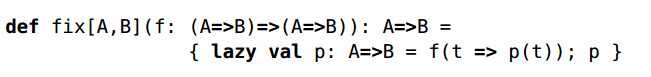
\includegraphics[width=0.9\textwidth]{Smolina/pics/fix.png}
\end{listing} 

Комбинирование элементарных анализаторов и представленных выше парсер-комбинаторов позволяет представить КС-грамматику и избежать зацикливания при использовании ~\cite{GLL}.

\subsection{Полный перебор с использованием Continuation-Passing Style}
У базовых распознавателей есть свои недостатки. Одна из проблем связана с тем, что работа распознавателя тесно связана с расположением правил в грамматике, первый распознаватель имеет более высокий приоритет. Например, когда распознавателю для грамматики $G_3$ (см. листиниг~\ref{grmG3}) будет представлена на вход строка “ab”, он вернёт $failure$. Это произойдет по причине того, что когда будет применен первый распознаватель из двух альтернативных, он распознает часть строки успешно, но дальнейшее распознавание завершиться ошибкой, и второй распознаватель так никогда и не будет применен к началу строки. Ещё одной проблемой базовых распознавателей является то, что результатом успешного распознавания всегда является единственное решение, когда как их может быть и несколько. Необходимо порождать все возможные выводы данной строки. Одним из подходов для решения этой задачи является техника Continuation-Passing
Style (CPS).

\begin{listing}
\caption{Грамматика $G_3$}
\label{grmG3}
\centering
$\begin{array}{rl}
A \rightarrow a \ | \ a \ b
\end{array}$
 \end{listing}

 Идея программирования в стиле Continuation-Passing состоит в том, что передача управления происходит через механизм продолжений.
Продолжение в данном контексте представляет собой состояние программы в конкретный момент времени, которое возможно сохранить и использовать для перехода в данное состояние.

Для того чтобы преобразовать базовые распознаватели в CPS авторы библиотеки Meerkat изменили тип $Result[T]$ и сопровождающие его функции $success$ и $failure$. Любой результат теперь должен быть представим как композиция двух функций, используя метод $flatMap$, или как комбинация двух возможных альтернатив – результатов, используя метод $orElse$. Реализация идеи в библиотеке Meerkat представлена на  листинге~\ref{result}.

\begin{listing}
\caption{Result[T] для CPS распознавателей}
\label{result}
\centering
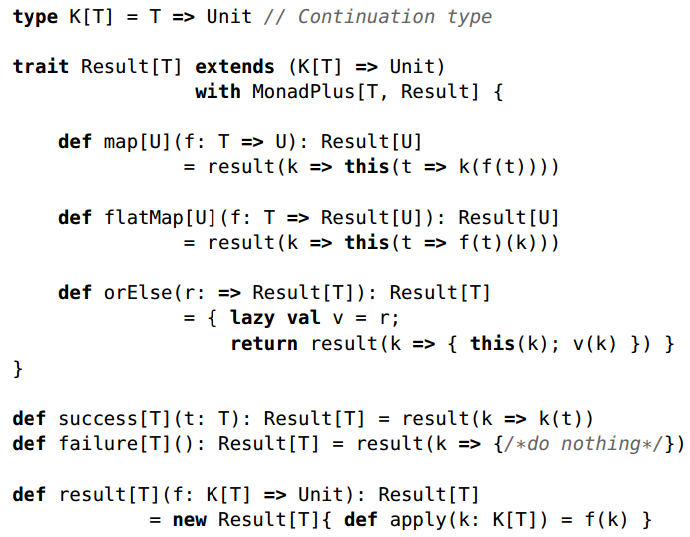
\includegraphics[width=0.8\textwidth]{Smolina/pics/result.png}
\end{listing}

CPS распознаватель принимает на вход позицию и возвращает функцию типа $Result[T]$. Данная функция принимает на вход продолжение типа $K[Int]$ и возвращает $Unit$. Продолжение в данном случае является функцией, которая представляет собой остаток от процесса распознавания. Вместо возвращения значения, распознаватель возвращает либо $success$, вызывая продолжение со следующей позицией, либо $failure$, не вызывая продолжения.

Таким образом, используя базовые распознаватели в терминах Continuation-Passing Style, авторами статьи~\cite{GLL} был получен полный перебор всех решений.

\subsection{Мемоизация и поддержка левой рекурсии}
Ранее были отмечены две проблемы у наивных реализаций парсер-комбинаторов – это проблема левой рекурсии и экспоненциального роста. Рассмотрим подробнее, как решены эти проблемы в библиотеке Meerkat. Проблема экспоненциального роста возникает при поиске всех деревьев разбора и связана с тем, что анализ входной последовательности распознавателем происходит без сохранения промежуточных результатов анализа.

Проблема левой рекурсии возникает с определенным типом грамматики (пример приведён на листинге~\ref{grmG2}). В представленном случае нетерминал бесконечно будет вызывает сам себя, так и не считав ни одного символа из входного потока. Такая ситуация может возникнуть либо явно,
либо когда префикс перед рекурсивным определением обращается в пустую строку.

В библиотеке Meerkat данные проблемы решаются мемоизацией и техникой CPS. Мемоизацией называют механизм, который позволяет сохранять вычисленные результаты и в дальнейшем переиспользовать их. При вычислении распознавателя, в первую очередь алгоритм смотрит на таблицу мемоизации и проверяет, не было ли вычислено значение данного распознавателя в данной позиции ранее. В случае, когда вычисление происходит в первый раз, результат работы распознавателя записывается в таблицу мемоизации. Иначе же распознаватель не вычисляется, а результат его работы берется из таблицы. На листинге~\ref{memo} представлен такой механизм для техники CPS, реализованный в библиотеке Meerkat.

 Функция $memo$ превращает произвольный распознаватель CPS в мемоизированный CPS-распознаватель. Мемоизированный CPS-распознаватель при каждом вызове в позиции i обращается к таблице $table$. Таблица $table$ содержит функцию для работы с продолжениями для каждого символа. В случае, когда для позиции i применяется немемоизированый распознаватель в первый раз, его модификация сохраняется и представляет собой переменную res. Результат распознавателя не вычисляется в тот же момент, а только после обновления таблицы table. Если распознаватель был вызван в данной позиции раньше, его результат возвращается из table и не перевычисляется. Таким образом решается проблема экспоненциального роста.

\begin{listing}
\caption{Мемоизация для CPS}
\label{memo}
\centering
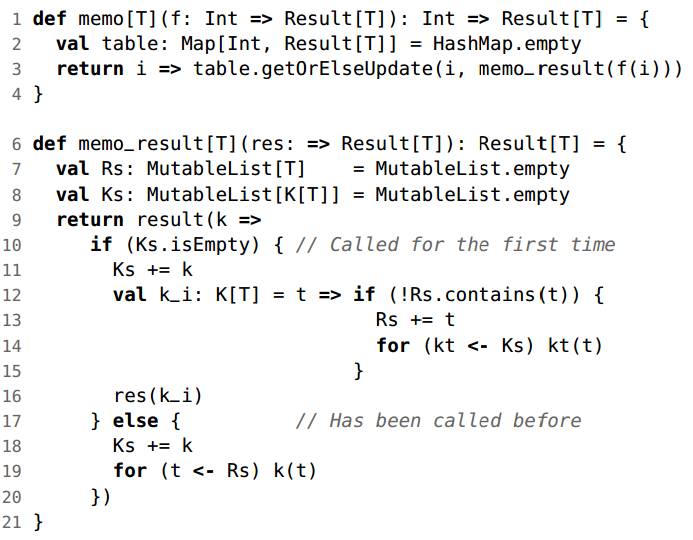
\includegraphics[width=0.8\textwidth]{Smolina/pics/memo.png}
\end{listing}

CPS-распознаватель имеет доступ к двум списками $Rs$ и $Ks$. Список $Rs$ содержит все позиции входа, созданные немемоизированным распознавателем, когда он достигает успеха в позиции $i$. Список $Ks$ содержит все продолжения, которые передаются в функцию $memo\_result$, когда они вызываются в позиции $i$. Если мемоизированный результат вызывается в первый раз, текущее продолжение добавляется к $Ks$, а исходный немемоизованный результат вызывается с новым продолжением $k\_i$. Продолжение $k\_i$ создается только после первого вызова мемоизированного распознавателя в $i$. Каждый раз, когда немемоизированный распознаватель завершается с успехом в позиции $i$, $k\_i$ проверяет, была ли эта входная позиция получена как результат раньше, если нет, сначала записывает ее в $Rs$, а затем запускает все записанные продолжения. С другой стороны, если вызванный мемоизированный результат был вызван ранее, текущее
продолжение $k$ добавляется к $Ks$ и вызывается для каждой входной позиции,записанной в $Rs$.

Теперь, когда мемоизированный леворекурсивный CPS-распознаватель вызывается во входной позиции $i$, его завершение гарантируется, поскольку соответствующий немемоизированный распознаватель никогда не будет вызван в $i$ более одного раза. В то же время часть пути выполнения, которая привела к леворекурсивному вызову и может создавать новые позиции ввода для левого рекурсивного распознавателя в $i$, эффективно записывается как продолжение. Каждое продолжение фиксирует следующий шаг в альтернативе после того, как текущий вызов возвращается. Продолжения будут выполняться для любой входной позиции, создаваемой леворекурсивным распознавателем в точке $i$, до тех пор, пока создаются новые позиции ввода~\cite{IzmCombinator}. Таким образом решается проблема левой рекурсии.

\subsection{ Библиотека для синтаксического анализа графов}
Основной задачей работы является разработка решения для синтаксического анализа графа, которое бы позволило не только писать запросы непосредственно в коде программы, но и получать результат этих запросов в компактной форме SPPF.

Данная работа требует решения промежуточных шагов:
\begin{enumerate}
\item входным типом данных библиотеки Meerkat являются строки, необходимо изменить его на граф;
\item строки можно рассматривать как линейную последовательность ребер и вершин, необходимо преобразовать библиотеку до того, чтобы стало возможным анализировать последовательность вершин с несколькими исходящими ребрами (деревья) с различными метками, а так же граф с циклами;
\item необходимо преобразовать библиотеку до того, чтобы стало возможным анализ графов с одинаковыми ребрами из одной вершины;
\item необходимо добавить функциональность для решения частных задач синтаксического анализа;
\item необходимо добавить функциональность для работы с графовойбазой данных Neo4j.
\end{enumerate}

\subsubsection{Изменение входного типа данных на граф}


Входной последовательностью в библиотеке Meerkat являются строки. Для работы с ними разработчиками библиотеки был разработан класс $Input$, который в конструкторе получает строку. Для добавления нового типа входных данных класс $Input$ был преобразован в интерфейс $Input$, который имеет следующие методы:
\begin{itemize}
\item $startWith$: принимает на вход строку $prefix$ и позицию в последовательности $n$. Проверяет, является ли prefix префиксом суффикса строки, начинающийся с позиции $n$;
\item $matchRegex$: принимает на вход регулярное выражение и позицию в последовательности. Проверяет, содержится ли в суффиксе строки с позиции $n$, строка удовлетворяющая данному регулярному выражению.
\end{itemize}

Класс $InputString$ реализует интерфейс для строки, класс $InputGraph$ – для графа. Для графа был разработан интерфейс $IGraph$, задающий методы необходимые для реализации класса $InputGraph$. Для тестирования данный интерфейс был реализован для типа данных $scalax.collection.Graph$~\cite{Graph}. Этопростоя в использовании реализация графа, в которой кратко и наглядно можно представить узлы и связи между ними.

\subsubsection{Преобразование системы для анализа дерева и графа с циклами}


Дерево представляет собой частный случай связного графа, в котором нет циклов. Пример дерева представлен на рис.~\ref{Graph1}. Обязательным условием на данном этапе является то, что метки на ребрах из одной вершины должны быть различны. Необходимо преобразовать библиотеку до того, чтобы стало возможным синтаксический анализ деревьев.

\begin{figure}

 \centering
 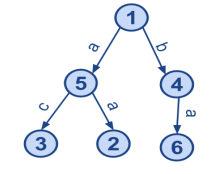
\includegraphics[width=0.4\textwidth]{Smolina/pics/Graph1.png}
 \caption{Дерево $A_1$}
 \label{Graph1}
\end{figure}

Для решения данной задачи необходимо обратить свое внимание на синтаксический анализатор терминала, реализованный в библиотеке Meerkat на листинге~\ref{parser1}. Данный метод принимает на вход некоторую строку, и позицию во входной последовательности. Если начиная с этой позиции существует подстрока, которая равна терминалу, то результат считается успешным и возвращается значение $success$, который содержит следующий символ, с которого следует продолжать разбор. 

В строке мы анализируем префикс длины $k$, начинающийся с позиции $n$ входного потока, в случае успеха, следующей позицией для анализа становится позиция $k+n$. В случае же с деревом это не верно. В дереве мы просматриваем все исходящие ребра, анализируем их на соответствии со значением терминал. Если для синтаксического анализатора существует ребро с соответствующим терминалом, для него следующей позицией становится номер вершины, в которую направлено ребро. Из чего следует, тип данных метода $startWith$ необходимо изменить с Boolean на $Option[Int]$.

Тип $Option$ является контейнером, энкапсулирующим понятие опционального значения. В случае успешного завершения, возвращается результат $Some(i)$, где $i$ – номер следующей вершины, или же $None$.

В графах с циклами, в отличие от деревьев, в одну и ту же вершину может существовать несколько путей, которые при этом могут образовывать циклы. В наивной реализации парсер-комбинаторов каждый путь приходилось бы пересчитывать заново, а в случае с циклом, вычисление бы никогда не завершилось. Однако применение техники мемоизации совместно с CPS позволяет избежать данных проблем. С использованием мемоизации вычисление каждого анализатора в каждой вершине происходит всего один раз. Для каждой вершины существует свой набор продолжений, который комбинируется и переиспользуется. Благодаря этим свойствам дальнейших изменений для поддержания графов с циклами не потребовалось. Циклы в графе обрабатываются подобно леворекурсивной грамматике.

Таким образом была решена задача синтаксического анализа для
деревьев и графов с циклами. Проиллюстрируем полученные результаты на примере 1.

\textsc{Пример 1.} 
Входной последовательностью является граф представленный на рис.~\ref{Graph2}. Данный граф цикличен. Из вершины 0 исходит
ребро с меткой «а» в вершину 1, а из вершины 1 исходит ребро с меткой «b». Стартовой вершиной считаем вершину 0. Проведем результат
синтаксического анализа в соответствии с грамматикой $G_4$ на рис.~\ref{grmG4}.

\begin{figure}
 \centering
 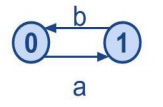
\includegraphics[width=0.2\textwidth]{Smolina/pics/Graph2.png}
 \caption{Цикличный граф $A_2$}
 \label{Graph2}
\end{figure}

\begin{listing}
\caption{Грамматика $G_4$}
\label{grmG4}
\centering
$\begin{array}{rl}
E \rightarrow a \ b \ E \ | \ a \ b
\end{array}$
 \end{listing}

\begin{figure}
 \centering
 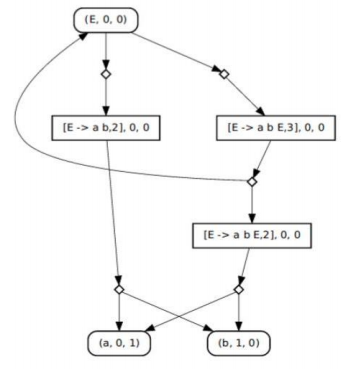
\includegraphics[width=0.4\textwidth]{Smolina/pics/Tree1.png}
 \caption{Результат работы синтаксического анализатора $E$ на
графе $A_2$}
 \label{Tree1}
\end{figure}

Результатом синтаксического анализа преобразованной библиотекой Meerkat является синтаксический лес разбора, представленый на рис~\ref{Tree1}. Из корневой вершины исходит две ветви, два возможных решения. Первое решение строка “ab”. Второе решение состоит из двух ветвей. Правая ветвь также конструирует строку “ab”, a левая ветвь указывает на корень дерева, это означает, что подстрока тоже должна принадлежать языку. Таким образом результатом анализа является бесконечное множество деревьев разбора.

\subsubsection{Преобразование системы для анализа графов с одинаковыми ребрами из одной вершины}


Ранее мы требовали, чтобы исходящие ребра имели уникальные метки. В этом случае из каждой вершины может существовать единственный путь, начинающийся с данного терминала. Если отказаться от данного ограничения, то таких путей может существовать несколько или не существовать вовсе. Итого, необходимо изменить тип и реализацию метода $startWith$. Теперь результатом его работы будет тип $Set[Int]$. Когда множество оказывается не пусто, будем считать, что разбор прошел успешно ($success$)
иначе не успешно ($failure$).

Метод $terminal$ также требует изменений. Все успешные пути, полученные методом $startWith$, комбинируются при помощи $orElse$ класса
$Result$. В результате чего получаем единственное продолжение, которое возвращается для дальнейшей обработки. Пример 2 демонстрирует работу новой реализации.

\textsc{Пример 2.} 
Входная последовательность – граф $A_3$ на рис.~\ref{Graph3}. Из стартовой вершины 0 исходят 3 ребра с одинаковыми метками. Проведем синтаксический анализ в соответствии с грамматикой $G_5$ на листинге~\ref{grmG5}.

\begin{figure}
 \centering
 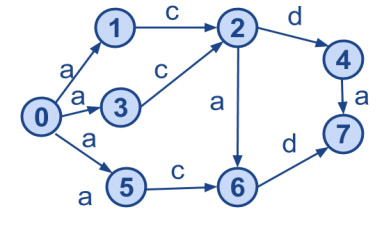
\includegraphics[width=0.6\textwidth]{Smolina/pics/Graph3.png}
 \caption{Граф $A_3$}
 \label{Graph3}
\end{figure}

\begin{listing}
\caption{Грамматика $G_5$}
\label{grmG5}
\centering
$\begin{array}{rl}
E \rightarrow a \ c \ d \ E \ | \ a \ d
\end{array}$
 \end{listing}

\begin{figure}
 \centering
 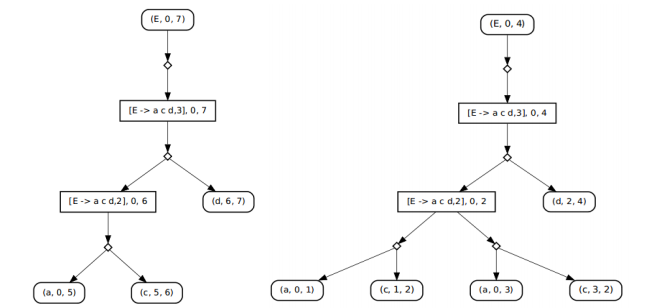
\includegraphics[width=\textwidth]{Smolina/pics/Trees2.png}
 \caption{– Результат работы синтаксического анализатора $E$ на графе $A_3$}
 \label{Trees2}
\end{figure}

Результат работы представлен на рис.~\ref{Trees2}. В графе $A_3$ из вершины 0 существуют 3 пути, соответствующие грамматике $G_5$ (0-5-6-7, 0-1-2-4 и 0-3-2-4). В результате получен граф SPPF, где несколько вершин выделены как начальные. Вершины, соответствующие общим подпутям при этом переиспользуются.

SPPF представляет собой компактное представление множества деревьев разбора одной строки. В случае синтаксического анализа графов необходимо построить множество деревьев разбора множества строк, что возможно сделать, если модифицировать SPPF таким образом, чтобы у него было несколько «корневых» узлов. За счет такого определения можно обеспечить переиспользование деревьев разбора для общих подпутей.

В библиотеке Meerkat во время анализа строится такая структура данных, как $SPPFLookup$. Она представляет собой множество уникальных узлов, создаваемых во время анализа, которые ссылаются друг на друга. При успешном результате один или несколько узлов, как в нашем случае, берутся как корни дерева.

\subsubsection{Функциональность для решения частных задач синтаксического анализа}


Раннее мы говорили о поиске всех путей в графе, удовлетворяющих заданным ограничениям. Существуют и другие семантики запросов, при которых необходимо идентифицировать некое подмножество всех путей, удовлетворяющих ограничениям. Такими семантиками являются~\cite{Hellings}:

\begin{itemize}
\item поиск всех путей в графе;
\item поиск путей, начинающихся с какой-либо вершины из данного
множества;
\item поиск путей, завершающихся в какой-нибудь вершине из данного
множества;
\item поиск путей, начинающихся в какой-нибудь вершине множества
начальных вершин и заканчивающихся в вершине из множества
конечных вершин.
\end{itemize}

Для того чтобы находить решения удовлетворяющие каждой из данных семантик, не нужно вносить изменений в процесс разбора. Задача решается благодаря структуре данных $SPPFLookup$, которая была описана выше. После конструирования $SPPFLookup$, необходимо лишь произвести фильтрацию стартовых нетерминальных символов, то есть выбрать корневые вершины, которые удовлетворяют требованиям. В итоге все вычисления производятся один раз и уже из полученных результатов выбираются необходимые.

\subsubsection{Интеграция библиотеки с графовой базой данных Neo4j}


После модификации библиотеки Meerkat для анализа графов, было решено применить результат работы на существующей графовой базе
данных. Нами была выбрана популярная графовая база данных Neo4j~\cite{Neo4j}. Она обладает наглядным и удобным в использовании интерфейсом, имеет REST API для доступа из любого языка программирования и большое количество пользователей по всему миру.

 Для интегрирования был реализован класс $Neo4jGraph$, реализующий методы интерфейса $IGraph$. Каждая вершина в графовой базе данных имеет свой уникальный идентификатор. Мы используем его как индекс во входном потоке. Класс использует REST API для работы с базой данных,предоставленное компанией Neo4j.

 \textsc{Пример 2.} 
Для тестирования была взята графовая база данных Wine. Фрагмент представлен на рис.~\ref{GraphWine}. Каждая вершина представляет собой вид вина, регион или тело вина. Между ними представлены два вида связи: 
\begin{itemize}
\item $locatedIn$ – указывает на расположение объекта, из которого
исходит ребро;
\item $hasBody$ – указывает на цвет вина
\end{itemize}

\begin{figure}
 \centering
 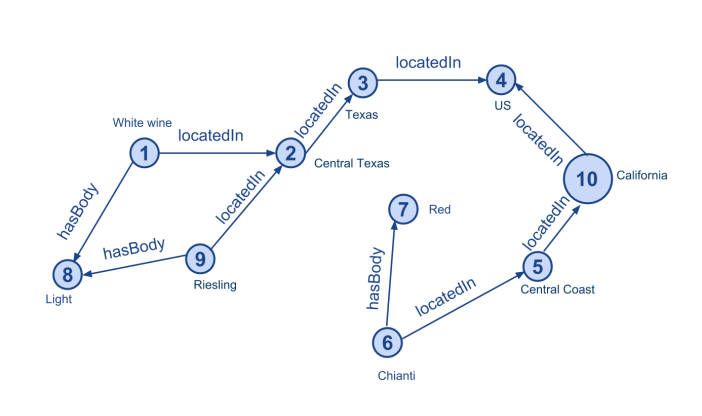
\includegraphics[width=0.9\textwidth]{Smolina/pics/GraphWine.png}
 \caption{Фрагмент графовой базы данных Wine}
 \label{GraphWine}
\end{figure}

Для того чтобы узнать в каких регионах производят Riesling, необходимо выполнить запрос представленный на листинге~\ref{grmG6}. 

\begin{listing}
\caption{Грамматика $G_6$}
\label{grmG6}
\centering
$\begin{array}{rl}
S \rightarrow locatedId \ S | \ locatedIn
\end{array}$
 \end{listing}

В процессе работы было получено 3 пути, начинающиеся с вершины 9 и заканчивающиеся в вершинах 2, 3, 4. Получив соответствующие этим вершинам названия, мы узнали расположение региона, где производится вино Riesling: Central Texas, Texas, US.
 
 \textsc{Пример 3.}

 Другой пример, демонстрирующий необходимость в запросах, представленных в КС-грамматиках, это поиск потомков одного
поколения.

База данных моделирует семейное древо (см. рис.~\ref{GraphFamily}). Требуется найти всех потомков одного поколения, например, все братьев и сестер конкретного узла. Нахождение всех этих потомков может быть произведено запросом в виде грамматики $G_7$ на листинге~\ref{grmG7}. Данная грамматика представляет собой язык правильных скобочных последовательностей, где одна скобка – ребенок, другой родитель. Технически данные в базе данных представлены только переходы от предков к потомкам, поэтому отношение «ребенок» необходимо симулировать как обратное ребро. Для обработки данной ситуации был добавлен комбинатор «not», который говорит о том, что анализ должен продолжаться в обратном направлении, от узла, в которое входит ребро, в узел, из которого исходит ребро.

\begin{figure}
 \centering
 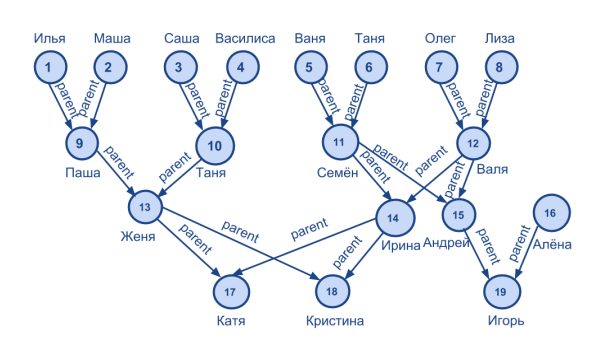
\includegraphics[width=0.8\textwidth]{Smolina/pics/GraphFamily.png}
 \caption{Фрагмент графовой базы данных «Семейное древо»}
 \label{GraphFamily}
\end{figure}

\begin{listing}
\caption{Грамматика $G_7$}
\label{grmG7}
\centering
$\begin{array}{rl}
S \rightarrow child \ S \ parent| \ epsilon
\end{array}$
 \end{listing}

 Найдем всех потомков одного поколения для Кати из базы данных «Семейное древо». Для этого запишем запрос в виде грамматики
представленной на листинге~\ref{grmG8}.

\begin{listing}
\caption{Грамматика $G_8$}
\label{grmG8}
\centering
$\begin{array}{rl}
S \rightarrow - \ parent \ S \ parent| \ epsilon
\end{array}$
 \end{listing}

 На выходе работы синтаксического анализатора было получено три дерева: дерево из вершины 17 в вершину 17, из 17 в 18 и из 17 в 19. Это
говорит о том, что в одном поколении находятся Катя, Кристина и Игорь. Так же из полученных деревьев можно узнать, кто является ближайшим общим родственником.
